\documentclass[a4paper,12pt]{article} % добавить leqno в [] для нумерации слева
\usepackage[a4paper,top=1.3cm,bottom=2cm,left=1.5cm,right=1.5cm,marginparwidth=0.75cm]{geometry}
%%% Работа с русским языком
\usepackage{cmap}					% поиск в PDF
\usepackage[warn]{mathtext} 		% русские буквы в фомулах
\usepackage[T2A]{fontenc}			% кодировка
\usepackage[utf8]{inputenc}			% кодировка исходного текста
\usepackage[english,russian]{babel}	% локализация и переносы
\usepackage{physics}
\usepackage{multirow}

%%% Нормальное размещение таблиц (писать [H] в окружении таблицы)
\usepackage{float}
\restylefloat{table}

\usepackage{graphicx}
\usepackage{wrapfig}
\usepackage{tabularx}

\usepackage{hyperref}
\usepackage[rgb]{xcolor}
\hypersetup{
	colorlinks=true,urlcolor=blue
}
\usepackage{pgfplots}
\pgfplotsset{compat=1.9}
%%% Дополнительная работа с математикой
\usepackage{amsmath,amsfonts,amssymb,amsthm,mathtools} % AMS
\usepackage{icomma} % "Умная" запятая: $0,2$ --- число, $0, 2$ --- перечисление

%% Номера формул
%\mathtoolsset{showonlyrefs=true} % Показывать номера только у тех формул, на которые есть \eqref{} в тексте.

%% Шрифты
\usepackage{euscript}	 % Шрифт Евклид
\usepackage{mathrsfs} % Красивый матшрифт

%% Свои команды
\DeclareMathOperator{\sgn}{\mathop{sgn}}

%% Перенос знаков в формулах (по Львовскому)
\newcommand*{\hm}[1]{#1\nobreak\discretionary{}
	{\hbox{$\mathsurround=0pt #1$}}{}}

\date{\today}

\begin{document} 
\begin{titlepage}
\begin{center}
		\textit{\large {Федеральное государственное автономное образовательное\\ учреждение высшего образования} }
		\vspace{0.5ex}
			
		\textbf{\large {«Московский физико-технический институт\\ (национальный исследовательский университет)»}}
	\end{center}
	\vspace{10ex}
	\begin{center}
		\vspace{13ex}
		\textbf{\Large {Лабораторная работа №4.1.2}}
			
		\Large{на тему:}
		\vspace{1ex}
			
		\textbf{\Large {Моделирование оптических приборов и определение их увеличения}}
			
		\vspace{42ex}
		\begin{flushright}
			\noindent
			\textit{Работу выполнили:}
			\\
			\textit{Сафин Дим\\ Сенокосов Арсений\\ группа Б02-012}
		\end{flushright}
		\vfill
		г. Долгопрудный \\2021 год
	\end{center}
\end{titlepage}

\textbf{Цель работы:} Определить фокусные расстояния собирающих и рассеивающих линз, смоделировать ход лучей в трубе Галилея, трубе Кеплера и микроскопе, определить их увеличение.\\
\textbf{В работе используются:} Оптическая скамья, набор линз, экран, осветитель со шкалой, зрительная труба, диафрагма, линейка.

\section*{Определение фокусных расстояний линз с помощью зрительной трубы}
\subsection*{Знакомство с линзами}
Рассмотрим доступные нам лизны и определим, какие из них являются собирающими, а какие --- рассеивающими. Для этого посветим параллельным пучком света через линзу и определим, наблюдается ли изображение (тогда линза положительная) и где (это будет фокус линзы). Для положительных также прикинем фокусное расстояние.
\par Получаем, что линзы 1-4 --- собирающие, а 5 --- рассеивающая. \par
\begin{center}
    $f_1 = 7.5$ см \hspace{1cm}  $f_2 = 10$ см \hspace{1cm}  $f_3 = 16$ см\hspace{1cm}  $f_4 = 30$ см
\end{center}

\subsection*{Определение фокусного расстояния собирающих линз}

\begin{enumerate}
    \item Настроим зрительную трубу на бесконечность
    \item Поставим положительную линзу на
расстоянии от предмета примерно равном фокусному. На небольшом расстоянии от линзы закрепим трубу, настроенную на бесконечность,
и отцентрируем её по высоте. Диафрагма диаметром
d = 1 см, надетая на ближнюю к осветителю линзу, уменьшит сферические аберрации и повысит чёткость изображения. \par
Передвигая линзу вдоль скамьи, получим в окуляре зрительной трубы изображение предмета
— миллиметровой сетки. При этом расстояние между предметом и серединой тонкой линзы (между проточками на оправах) равно фокусному.
    \item Результаты измерения фокусных расстояний собирающих линз:
\begin{table}[H]
	\caption{Фокусные расстояния собирающих линз в зависимости от стороны}
	\label{table1}	
	\begin{center}
		\begin{tabular}{|c|c|c|c|c|}
			\hline
			Сторона   & $ f_1,$ cм & $ f_2 $, см & $f_3 $, cм & $ f_4 $, cм\\
			\hline
			front &	 $7.7\pm0.5$	&	$9.2\pm0.5$   & $17.3\pm0.5$  & $32.3\pm0.5$ \\
			\hline
			back  &	$7.8\pm0.5$	&	$10.6\pm0.5$  & $16.5\pm0.5$  & $32.2\pm0.5$ \\
			\hline
		\end{tabular}
	\end{center}

\end{table}
\end{enumerate}

\subsection*{Определение фокусного расстояния рассеивающих линз}
\begin{enumerate}
    \item Для определения фокусного расстояния тонкой отрицательной линзы сначала получим на экране увеличенное изображение сетки при помощи одной короткофокусной положительной линзы. Измерим расстояние между линзой и экраном: $a_0 = 33.2$ см.
    \item Разместим сразу за экраном трубу, настроенную на бесконечность, и закрепим её. Уберём экран и поставим на его место исследуемую рассеивающую линзу (рис. 8). Перемещая рассеивающую линзу, найдём в окуляре зрительной трубы резкое изображение сетки. \par
    Измерив расстояние между линзами $l = 25.1$ см, рассчитаем фокусное расстояние рассеивающей линзы $f = a_0 - l$.
    \item Результаты измерения фокусного расстояния рассеивающих линз:
    \begin{center}
        $|f_5| = (8.1\pm0.5) $ см
    \end{center}
\end{enumerate}

\begin{figure}[h]
\begin{center}
\begin{minipage}[h]{0.40\linewidth}
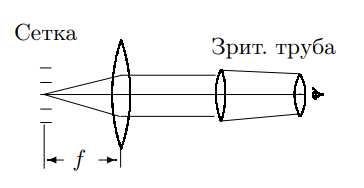
\includegraphics[width=1\linewidth]{plus_lens.PNG}
\caption{Определение фокусного расстояния собирающей линзы} %% подпись к рисунку
\label{ris:experimoriginal} %% метка рисунка для ссылки на него
\end{minipage}
\hfill 
\begin{minipage}[h]{0.40\linewidth}
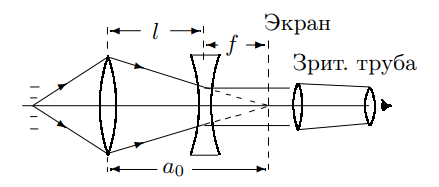
\includegraphics[width=1\linewidth]{minus_lens.PNG}
\caption{Определение фокусного расстояния рассеивающей линзы}
\label{ris:experimcoded}
\end{minipage}
\end{center}
\end{figure}

\section*{Моделирование трубы Кеплера}
\begin{enumerate}
    \item Рассмотрим ход лучей в трубе Кеплера и найдём увеличение данной оптической системы:
    
    \begin{figure}[h]
    \centering
    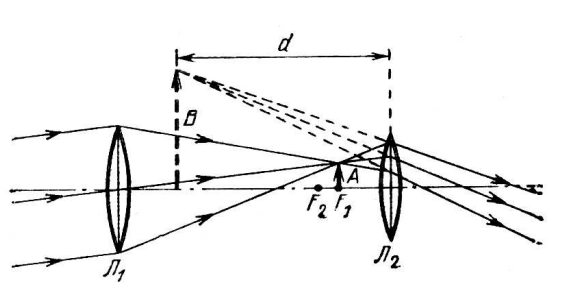
\includegraphics[width=9cm]{kepler.PNG}
    \caption{Ход лучей в трубе Кеплера}
    \label{fig:vac}
\end{figure}

Пусть пучок света, попадающий в объектив, составляет с оптической осью угол $\varphi_1$, а пучок, выходящий из окуляра, — угол $\varphi_2$. Увеличение $\gamma$ зрительной трубы по определению равно
\begin{equation}
    \gamma = \frac{\tan \varphi_2}{\tan \varphi_1},
\end{equation}
но также из рис. 3 следует, что 
\begin{equation}
    \gamma_K = -\frac{f_1}{f_2} = -\frac{D_1}{D_2},
\end{equation}
где $D_1$ - ширина пучка, прошедшего через объектив, а $D_2$ - ширина пучка, вышедшего из окуляра

\item Построим оптическую систему из каллиматора и непосредственно трубы Кеплера. 

    \begin{figure}[h]
    \centering
    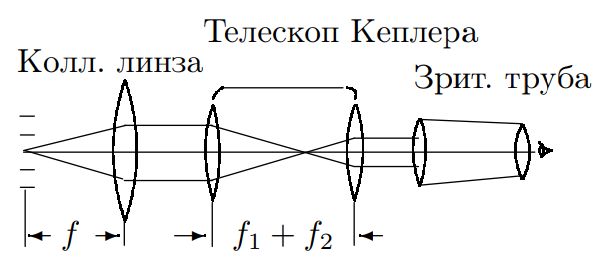
\includegraphics[width=9cm]{kepler_2.PNG}
    \caption{Схема трубы Кеплера}
    \label{fig:vac}
\end{figure}

Параметры действующих линз:
\begin{center}
    $ f_2 = (9.2\pm0.5) $ см \hspace{1cm} $f_4 = (32.2\pm0.5) $ см
\end{center}

Найдём увеличение трубы Кеплера непосредственно: пусть $h_1$ - размер ячейки миллиметровой сетки без телескопа, $h_2$ - с телескопом
\begin{center}
$h_1 = (10 \pm 1)$ дел., \hspace{1cm} $h_2 = (36 \pm 1)$ дел.
\end{center}
\[\boxed{\normalsize\gamma_K = -\frac{h_2}{h_1} = -3.6 \pm 0.4} \]


Также увеличение телескопа можно определить посредством сравнения диаметры оправы его объектива и диаметра изображения этой оправы в окуляре.
\begin{center}
	$D_1 = (3.6 \pm 0.2)$ см, \hspace{1cm} $D_2 = (12.8 \pm 0.2)$ см
\end{center}
\[\boxed{\normalsize\gamma_K = -\frac{D_2}{D_1} = -3.5 \pm 0.3} \]


При этом по формуле (2) также
    \[ \boxed{\gamma_K = -\frac{f_1}{f_2} = -3.5 \pm 0.1} \] 


Полученные значения совпадают в пределах погрешности.
\end{enumerate}

\section*{Моделирование трубы Галилея}
    \begin{figure}[h]
    \centering
    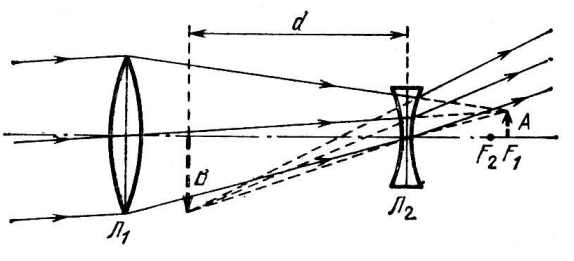
\includegraphics[width=9cm]{gal.PNG}
    \caption{Ход лучей в трубе Галилея}
    \label{fig:vac}
\end{figure}

\begin{enumerate}
    \item Труба Галилея получается из трубы Кеплера заменой собирающей линзы окуляра рассеивающей. Формулы для увеличения, соответственно, остаются теми же:
\begin{equation}
    \gamma_G = -\frac{f_1}{f_2} = -\frac{D_1}{D_2},
\end{equation}

\item Заменим собирающую линзу с фокусным расстоянием $ f_2 = 9.2 $ см рассеивающей с фокусным расстоянием $ |f_5| = 8.1 $ см. Проведём те же операции, что и для трубы Кеплера:

\begin{center}
$h_1 = (10 \pm 1) $ дел., \hspace{1cm} $h_2 = (41 \pm 1) $ дел. \par
\[ \boxed{\gamma_K = -\frac{h_2}{h_1} = -4.1 \pm 0.4} \]
\end{center}

При этом по формуле (2) также
\begin{center}
    \[ \boxed{\gamma_K = -\frac{f_1}{f_2} = -4.0 \pm 0.2} \]
\end{center}

Полученные значения вновь совпадают в пределах погрешности.
\end{enumerate}

\section*{Моделирование микроскопа}

    \begin{figure}[h]
    \centering
    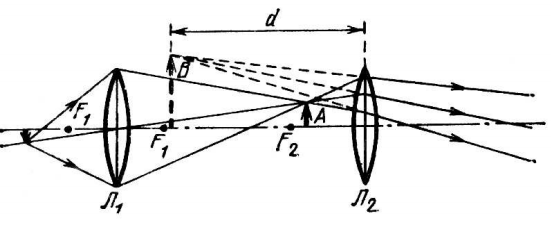
\includegraphics[width=9cm]{micro.PNG}
    \caption{Ход лучей в микроскопе}
    \label{fig:vac}
\end{figure}

\begin{enumerate}
    \item Ход лучей в микроскопе показан на рис. 6. Увеличение микроскопа вычисляется по формуле
    \begin{equation}
        \gamma_M = \Gamma_{ob} \Gamma_{oc} = -\frac{\triangle}{f_1} \frac{L}{f_2},
    \end{equation}
    где $f_1$ и $f_2$ - фокусные расстояния линз микроскопа, $\triangle = l_{12}-f_1-f_2$ см - интервал, $ l_{12} $ -- длина тубуса, $L$ - расстояние наилучшего зрения ($L = 25$ см).
    
    \begin{figure}[h]
    \centering
    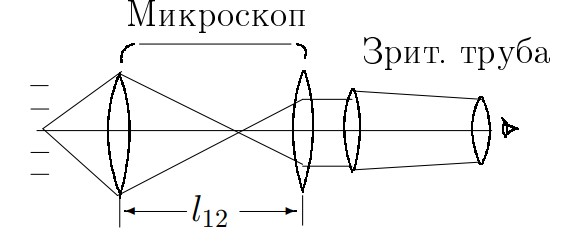
\includegraphics[width=9cm]{micro.jpg}
    \caption{Схема микроскопа}
    \label{fig:vac}
\end{figure}    
    
     Соберём микроскоп с пятикратным увеличением. Используемые линзы: $f_1 = 7.7 $ см, $ f_2 = 9.2 $ см. Получим
        \[ \gamma_M^\text{теор} = -\frac{\triangle}{f_1} \frac{L}{f_2} = -5 \]
    Исходя из этого получим необходимую длину тубуса $ l_{12} = 32.5 $ см.
    Проводя измерения угловых размеров миллиметровой сетки для такой конфигурации имеем $ h_2 = 36\pm1 $. Тогда
        \[ \boxed{\gamma_M^\text{эксп} = -\frac{h_2L}{h_1f} = -5.18 \pm 0.15} \]
        где $ f $ -- фокусное расстояние линзы-коллиматора из п.2, $ f = f_3 = 17.3 $ см.

Значения совпадают в пределах погрешности.
\end{enumerate}

\section*{Вывод}
В ходе выполнения лабораторной работы были получены следующие результаты:

\begin{itemize}
	\item Сначала при помощи поиска действительного изображения осветительного прибора в линзе было определен их тип. В итоге получилось, что линзы 1-4 -- собирающие, а 5 -- рассеивающая. Также <<на глаз>> было оценено их фокусное расстояние.
	\begin{center}
		$f_1 = 7.5$ см \hspace{1cm}  $f_2 = 10$ см \hspace{1cm}  $f_3 = 16$ см\hspace{1cm}  $f_4 = 30$ см
	\end{center}
	\item В дальнейшем фокусное расстояние линз было определено точно при помощи зрительной трубы, настроенной на бесконечность. В итоге получаем следующие результаты:
	\begin{center}
		$f_1 = (7.8 \pm 0.6)$ см \hspace{1cm}  $f_2 = (9.9\pm0.6)$ см \hspace{1cm}  $f_3 = (16.9 \pm 0.6)$ см\hspace{1cm}  $f_4 = (32.3 \pm 0.6)$ см \hspace{1cm}  $f_5 = (-8.1 \pm 0.6)$ см
	\end{center}
	\item При моделировании оптических приборов было экспериментально измерено их увеличение, а затем сравнено с теоретическими значениями. Так, например, для трубы Кеплера имеем
	\[\gamma_K^\text{угл} = -\frac{h_2}{h_1} = -3.6 \pm 0.4 \]
	\[\gamma_K^\text{диам} = -\frac{h_2}{h_1} = -3.5 \pm 0.3 \]
	\[\gamma_K^\text{теор} = -\frac{h_2}{h_1} = -3.5 \pm 0.1 \]
	По результатам измерений можно сделать вывод о их совпадении в пределах погрешности.
	\item Такие же измерения проведены и для модели трубы Галилея. В итоге получены следующие результаты.
	\[\gamma_K^\text{угл} = -\frac{h_2}{h_1} = -4.1 \pm 0.4 \]
	\[\gamma_K^\text{теор} = -\frac{h_2}{h_1} = -4.0 \pm 0.2 \]
	\item Также в ходе выполнения лабораторной работы была собрана модель микроскопа с планируемым теоретическим увеличением $  \gamma_M^\text{теор} = 5 $. В ходе эксперимента было получено следующее реальное значение увеличение микроскопа:
	\[ \gamma_M^\text{эксп} = -\frac{h_2L}{h_1f} = -5.18 \pm 0.15 \]
	Некоторое расхождение с теорией объясняется неточностью при выставлении приборов на оптической скамье, в особенности их продольных сдвигов.
\end{itemize}

\end{document}